\documentclass[conference]{IEEEtran}
\IEEEoverridecommandlockouts
% The preceding line is only needed to identify funding in the first footnote. If that is unneeded, please comment it out.
\usepackage{cite}
\usepackage{amsmath,amssymb,amsfonts}
\usepackage{algorithmic}
\usepackage{float}
\usepackage{graphicx}
\usepackage{textcomp}
\usepackage{xcolor}
\newcommand{\argmax}[1]{\underset{#1}{\operatorname{arg}\,\operatorname{max}}\;}
\newcommand{\argmin}[1]{\underset{#1}{\operatorname{arg}\,\operatorname{min}}\;}
\def\BibTeX{{\rm B\kern-.05em{\sc i\kern-.025em b}\kern-.08em
    T\kern-.1667em\lower.7ex\hbox{E}\kern-.125emX}}
\begin{document}

\title{Application of Partile Filter in Simultaneous Localization and Mapping}


\author{\IEEEauthorblockN{Joseph Bell}
\IEEEauthorblockA{\textit{Department of Electrical and Computer Engineering} \\
\textit{University of California, San Diego}\\
jjbell@eng.ucsd.edu}
}

\maketitle

\begin{abstract}
This paper presents an approach to simultaneous localization and mapping (SLAM) by use of a particle filter in conjunction with lidar and odometry data. The SLAM approach was tested in five independent environments. The results of this SLAM approach were satisfactory in regard to visual representations of the mapped environment and movement prediction of the robot. However, the success of the algorithm varied by environment.
\end{abstract}

\begin{IEEEkeywords}
SLAM, particle filter
\end{IEEEkeywords}

\section{Introduction}

SLAM has a wide array of applications, from autonomous driving to to exploration of uncharted territories. SLAM is often considered a chicken and egg problem due to the dependency of localization and mapping on each other. If one knew the map then localization would be easy, and if one knew the location of the robot (i.e. there's no noise in the robot's movement) then creating a map would be easy. However, in cases where neither the map nor location of the system/robot are known, localization and mapping work simultaneously to gradually refine the robot/system position and environment. 

A current, real-life application of SLAM is Google's self driving car which uses a range finder to generate maps of it's environment - these maps are used in conjunction with it's previously generated maps of the world so that it can drive itself autonomously. In this case, SLAM helps Google's car navigate robustly without being thrown off by slight perturbations and new objects in the environment. The ability for robots to navigate in new environments is crucial for exploration as most of this planet (and other planets) is not habitable for humans. Robots have the ability to explore areas that are too dangerous for humans, and it is very tricky, if not impossible, for a robot to navigate in an environment that no human has been to before without the application of an algorithm like SLAM.

The goal of this paper is to detail an approach to SLAM using a particle filter in order to locate and map a robot in a series of hallways. The robot is equipped with lidar and odometry sensors on it's head, and it also has the ability to pitch and yaw it's head. A diagram of the robot can be seen in Figure 1.This paper will first introduce the problem formulation and will follow with an explanation of the technical approach and methods used to implement SLAM. Lastly, results of the particle filter application to SLAM will be presented and discussed.


\section{Problem Formulation}

\begin{figure}[H]
\centerline{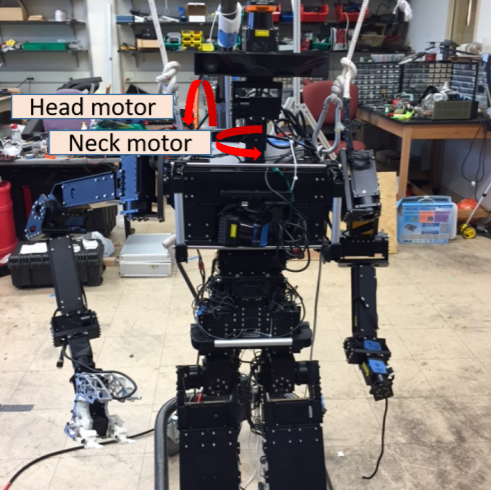
\includegraphics[width=50mm]{thor.png}}
\caption{Thor - the robot used for this paper}
\end{figure} 

Given a set of states $x_{0:T}$, controls $u_{0:t-1}$, and observations $z_{0:T}$ find solutions to the SLAM problem that use a motion model from the control inputs and an observation model from the observations to localize the robot and create a map (m) of the environment. One motion model should be developed that is then applied to all five environments.

Due to Markov assumptions, the joint pdf used for localization and mapping can be decomposed to:
\begin{figure}[H]
\centerline{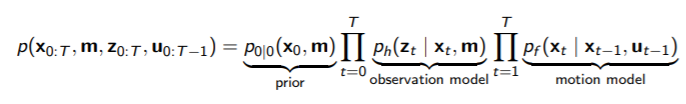
\includegraphics[width=90mm]{eq1.png}}
\end{figure} 



\section{Technical Approach}
The technical approach consists of four separate sub-problems that when put together generate SLAM solutions.
\subsection{Mapping}
 
The method for mapping was to create an occupancy grid that represents a pdf $p(m | z_{0:t}, x_{0:t})$ where the map cells $m_{i}$ are modeled as independent Bernoulli random variables:
\begin{figure}[H]
\centerline{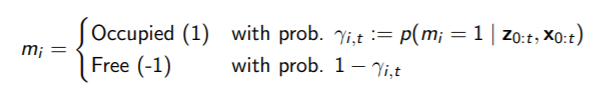
\includegraphics[width=90mm]{eq2.png}}
\end{figure} 

Based on the observations, the grid cells get updated with occupancy probabilities which ultimately becomes the accumulation of the log-odds ratio per map pixel $m_{i}$, with the odds ratio being represented as:

\begin{figure}[H]
\centerline{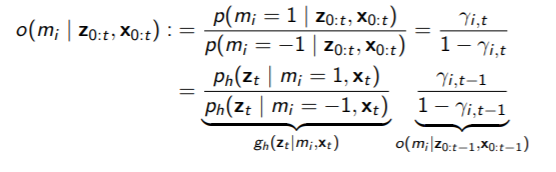
\includegraphics[width=90mm]{eq4.png}}
\end{figure} 

By using Bayes rule the odds ratio can be rewritten in terms of the observation model:

\begin{figure}[H]
\centerline{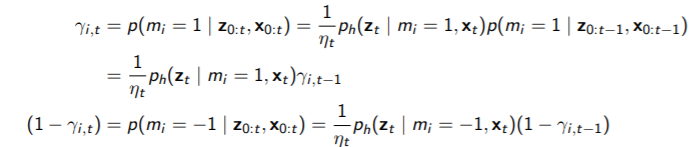
\includegraphics[width=90mm]{eq3.png}}
\end{figure} 

Next, as previously stated, the occupancy probabilities are simply the accumulation of the log-odds ratio:

\begin{figure}[H]
\centerline{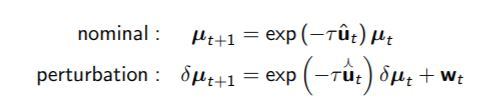
\includegraphics[width=90mm]{eq5.png}}
\end{figure} 

This reduces to simply keeping track of the cell log-odds of the map per time step:

\begin{figure}[H]
\centerline{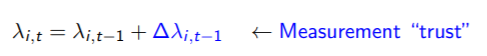
\includegraphics[width=70mm]{eq6.png}}
\end{figure} 

However, the measurement trust of the observation model needs to be determined. Bayes rule is applied once again to obtain:

\begin{figure}[H]
\centerline{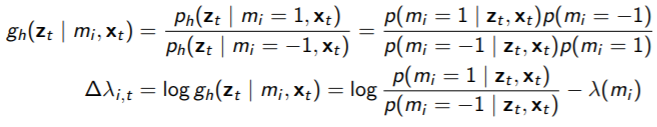
\includegraphics[width=70mm]{eq7.png}}
\end{figure} 

The first term is an inverse observation model that specifies how much to trust the observations. The second term is a prior occupancy log-odds ratio, and for this application it's chosen as 0. A value greater than 0 could be chosen if one is optimistic about free space, however since these maps are unknown there is no justified reason to be optimistic about free space. For the measurement trust a log ratio of 4 was used, represented as:

\begin{figure}[H]
\centerline{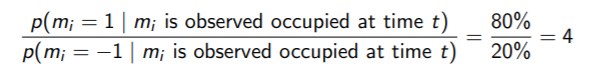
\includegraphics[width=70mm]{eq8.png}}
\end{figure} 

The next step is to actually apply these observation updates to a grid map of cells representing the environment. In order to do this, a series of transformations were required to transform the lidar data to world coordinates. Using the rotations of the robot's neck and head a rotation matrix was constructed (using Tait-Bryan angles) to relate the lidar coordinate frame to the body coordinate frame. A z-translation vector was also used to relate the lidar coordinate frame to the body coordinate frame. Using the odometer values, the pose of the robot in world coordinates was calculated and used to create a rotation matrix (using Tait-Bryan angles again) to relate the body coordinate frame to the world coordinate frame. An additional z-translation vector was used to relate the body coordinate frame to the world-coordinate frame. The conversion of lidar frame to body frame and then body frame to world frame ultimately results in the lidar scans represented in the world coordinate frame.


\begin{figure}[H]
\centerline{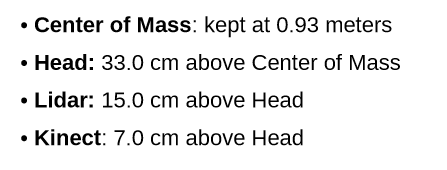
\includegraphics[width=50mm]{thor_datat.png}}
\caption{Location of Thor's sensors and center of mass}
\end{figure} 

Bresenham's line rasterization algorithm was used to determine all cells that each lidar scan passed through up until it hit an object. This last cell had it's log odds increased (as it represents the lidar scan being obstructed) and every other cell had it's log odds decreased. Lidar scans that hit below 10 centimeters in the world z-axis were omitted as these were likely to be scans reflecting off the ground. Also, as per the spec sheet of the lidar scanner it has a maximum range of 30 meters. Therefore, any scans greater than 29 meters were omitted as these are not going to be reliable measurements. The log odds values were constrained to a minimum and maximum value of -100 and 100 respectively to avoid overconfident estimation. The logic behind these limits was that since each lidar scan set consists of 1081 scans and each scan can attribute log(4) to a cell, this totals to approximately 650 "confidence units" per scan set.  It will take about 166 scans to fully flip the occupancy of a grid cell (100 units), which means it's quite unlikely to have 166 false positives or false negatives but also not too difficult to flip the occupancy of a grid cell if a future scan seems to thing it's state was wrong. 


\subsection{Prediction}

The robot's state was represented as a mixture of dirac-delta functions with corresponding weights - each dirac-delta function and its weight is referred to as a particle. Each particle originates from the world origin and has the motion model applied to it. All weights were initialized to $\frac{1}{N}$ where N is the number of particles. The motion model was determined by the odometry data that provided incremental changes in the x, y, and theta positions of the robot in the world coordinates (theta being counter-clockwise rotation about the z-axis). 

Noise was sampled from a Gaussian distribution using numpy's random.normal function. A series of approaches were taken to determine an adequate noise model of the robot's movement. One attempt at a noise model was taken to be a Gaussian distribution with 0 mean and standard deviation equal to 5 percent of the change in the robot's pose. The final noise model was taken to be a Gaussian distribution with 0 mean and standard deviation equal to 0.7, 0.7, and 0.2 respectively for the x, y, and theta components of the pose. Another variable that was modified often was the number of particles. It was tough to find a balance between accuracy and computational time, but a set of 200 particles proved to be acceptable and not too computationally expensive. This motion model proved to be the most robust for handling large and small perturbations in the pose. The final motion model for the particles can be represented as:

\begin{figure}[H]
\centerline{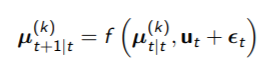
\includegraphics[width=30mm]{mm.png}}

where $\epsilon_{t}$ is Gaussian noise and $u_{t}$ is the pose update proved by the odometry readings.

\end{figure} 

\subsection{Update}

The pose of the robot was adjusted using a laser correlation model. Each particle's set of laser scans was converted to world coordinates and checked with the current map to check for correlation. The correlation for a particle is simply the number of lidar scans that correspond with the most recently updated map, as represented by the equation, where y is the scan in grid coordinates and m is the map:

\begin{figure}[H]
\centerline{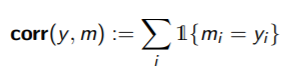
\includegraphics[width=40mm]{eq10.png}}
\end{figure}


The new weight of each particle corresponded to the soft max of it's correlation, as shown in the equation below:

\begin{figure}[H]
\centerline{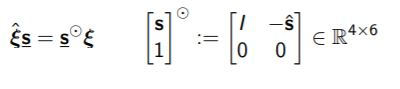
\includegraphics[width=50mm]{eq9.png}}
\end{figure} 

\subsection{Resampling}

The number of effective particles was calculated via the equation:

\begin{figure}[H]
\centerline{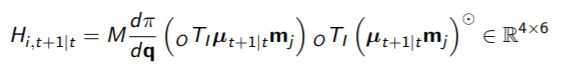
\includegraphics[width=30mm]{eq11.png}}
\end{figure} 

When the number of effective particles passed below a threshold the particles were resampled and the weights were reset back to the prior of $\frac{1}{N}$ were N is the number of particles. The threshold for this application was set at 20\% of the number of particles. The resampling used for this application was Monte Carlo sampling from the filterpy python module. An example of resampled particles that was triggered by particle depletion can be observed in Figure 3.
\begin{figure}[H]
\centerline{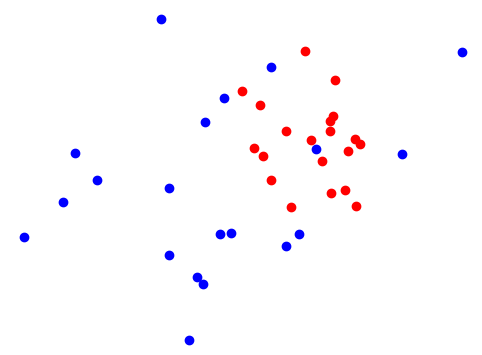
\includegraphics[width=30mm]{resample.png}}
\caption{Resampled particles (red = resampled, blue = original)}
\end{figure} 




\section{Results and Discussion}
The SLAM approach was applied to 5 separate data sets - all the results can be seen at the end of this section (images are flipped between dead reckoning and particle filter). 

The maps generated are respectable in the sense that they do resemble hallways (the environment the robot was placed in). However they are not as clean looking as I had hoped. Attempts made to clean up the results were: changing the noise variance, increasing the number of particles, modifying the height to cut off scans of the floor, modifying the lidar distance cut off range, and modifying the upper and lower limits of the cell log-odds. A noise variance too large in magnitude resulted in chaotic maps, and too low of a noise variance proved no better than dead-reckoning. The hardest factor to accommodate for was larger robot rotations - unexpectedly, neither increasing the number of particles nor increasing the noise variance helped this issue (most of the time the variance increase made the maps worse).

The difference between my dead reckoning and particle filter plots is not too impressive. I'm quite sure that there should be much more improvement between the two approaches, however after days of debugging I am unable to figure out a fix.


One aspect of the project that was difficult was managing the size of the data. There was a large amount of data to be processed, so code optimization was very important. One of the methods used to handle the data was to down sample it for quick debugging. However, down sampling would result in larger pose changes and thus would affect the noise distribution that was created as a function of the change in pose. Therefore, it was difficult to find a motion model incorporating noise for the full data set due to the immense amount of time required to process the data and the motion model used for the down sampled data did not necessarily translate to the full data set. This is the reason that the motion model resulted in constant variance values for the noise distribution. Unfortunately, due to time constraints, the plots all result from down sampling. I had spent too long trying to modify code to obtain better results and needed to downsample data (by a factor of 10, as opposed to 100 used for debugging) to obtain plots in time to meet the project deadline.

Another major aspect of this project that I believe would help future students is to provide more in depth documentation on the provided utility functions and data along with more description on the objective of the project. A large portion of time was spent figuring out what the data represented and how to get started on the project, and with more documentation this would not have been as big of an issue.

The trajectory plots were almost identical between dead reckoning and particle filter so only particle filter plots were included. 

If more time was allotted I would continue to explore the relationship between noise and my outputs. The hard thing about testing variance values is the amount of time required to see the results of variance changes. The attached code clearly outlines the steps taken for this algorithm and any feedback regarding where issues may lie would be greatly appreciated - either by being posted on Piazza for the course or by being directly emailed to me.

\begin{figure}[H]
\centerline{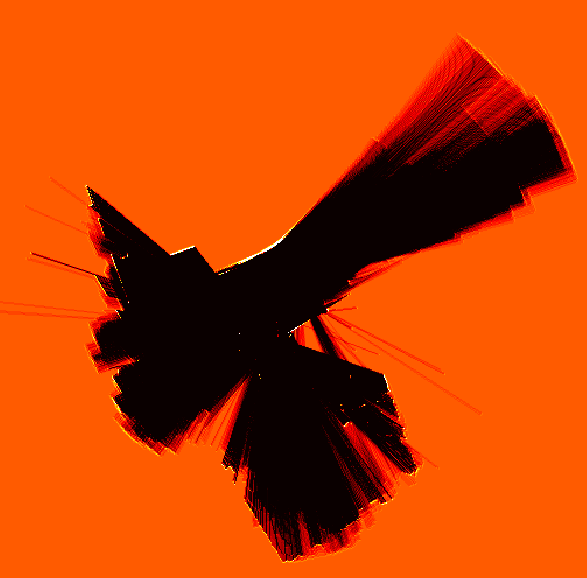
\includegraphics[width=30mm]{l0_logmap.png}}
\caption{Dead reckoning for environment 1}
\end{figure} 
\begin{figure}[H]
\centerline{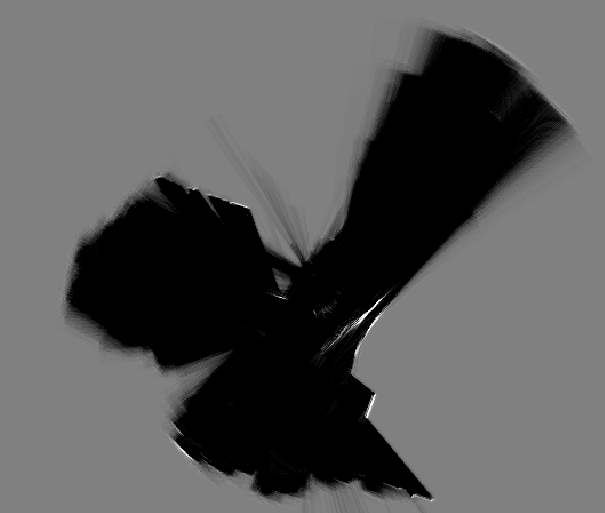
\includegraphics[width=30mm]{l0_particle.png}}
\caption{Particle filter for environment 1}
\end{figure}

\begin{figure}[H]
\centerline{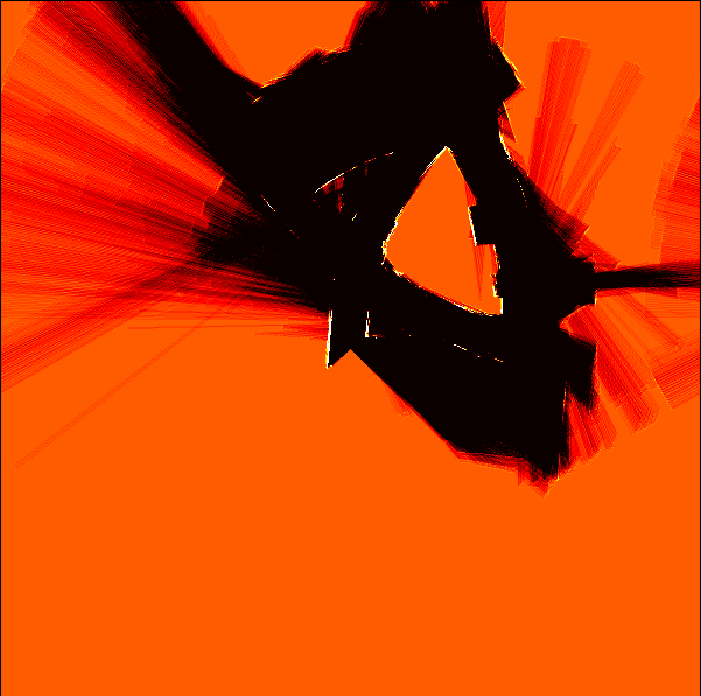
\includegraphics[width=30mm]{l1_logmap.png}}
\caption{Dead reckoning for environment 2}
\end{figure} 
\begin{figure}[H]
\centerline{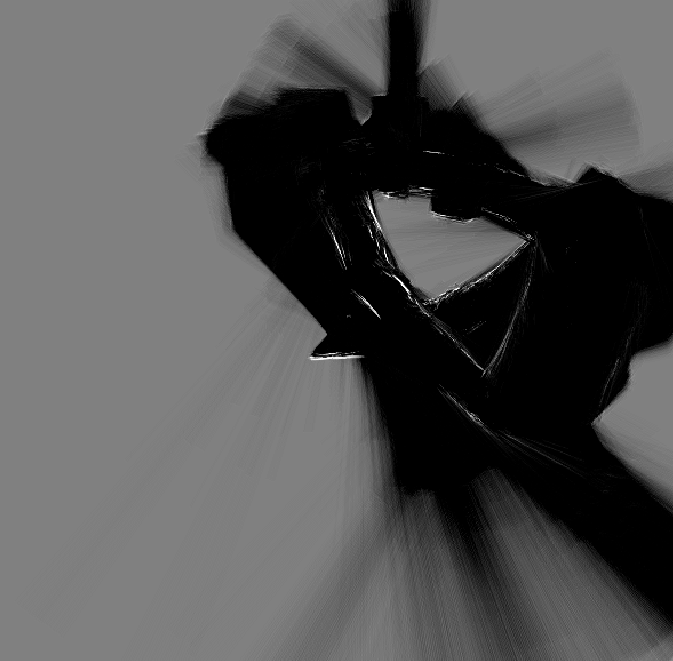
\includegraphics[width=30mm]{l1_particle.png}}
\caption{Particle filter for environment 2}
\end{figure}

\begin{figure}[H]
\centerline{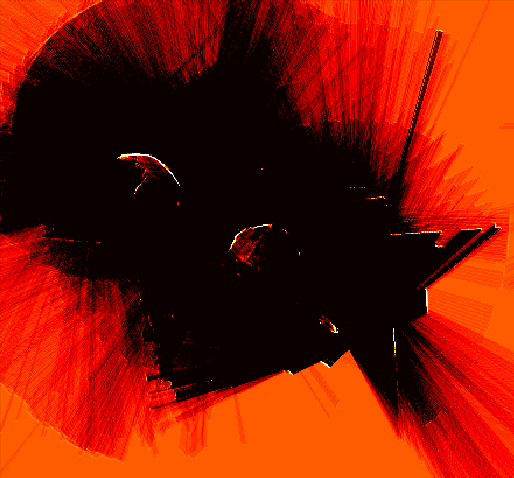
\includegraphics[width=30mm]{l2_logmap.png}}
\caption{Dead reckoning for environment 3}
\end{figure} 
\begin{figure}[H]
\centerline{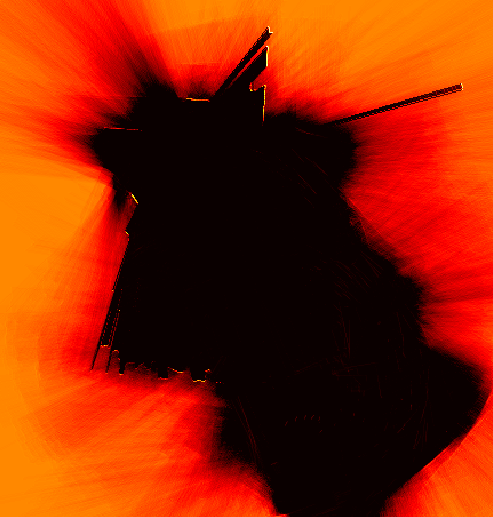
\includegraphics[width=30mm]{l2_particle.png}}
\caption{Particle filter for environment 3}
\end{figure}

\begin{figure}[H]
\centerline{
\includegraphics[width=30mm]{l3_logmap.png}}
\caption{Dead reckoning for environment 4}
\end{figure} 
\begin{figure}[H]
\centerline{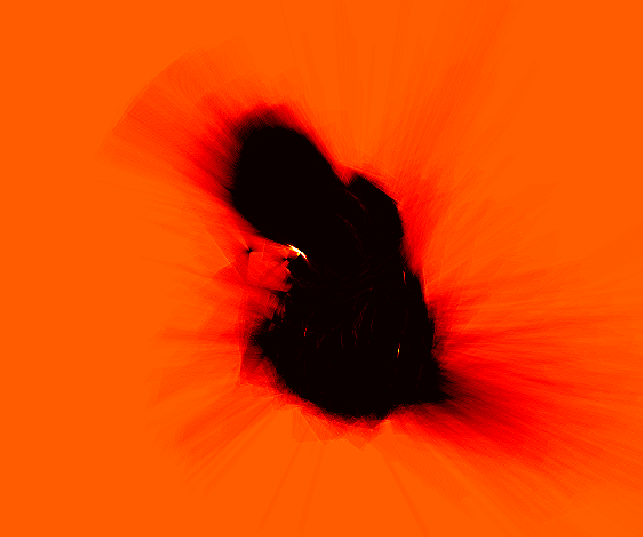
\includegraphics[width=30mm]{l3_particle.png}}
\caption{Particle filter for environment 4}
\end{figure}

\begin{figure}[H]
\centerline{
\includegraphics[width=30mm]{l4_logmap.png}}
\caption{Dead reckoning for environment 5}
\end{figure} 
\begin{figure}[H]
\centerline{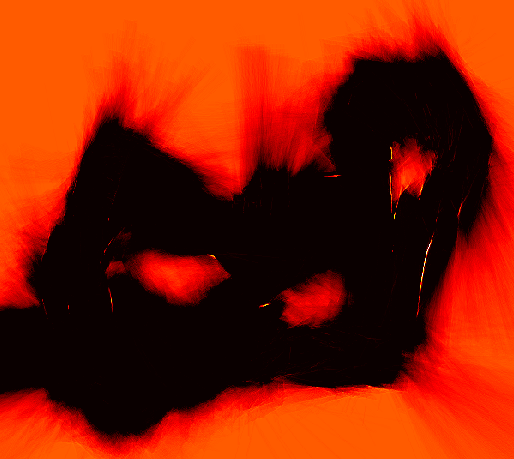
\includegraphics[width=30mm]{l4_particle.png}}
\caption{Particle filter for environment 5}
\end{figure}

\begin{figure}[H]
\centerline{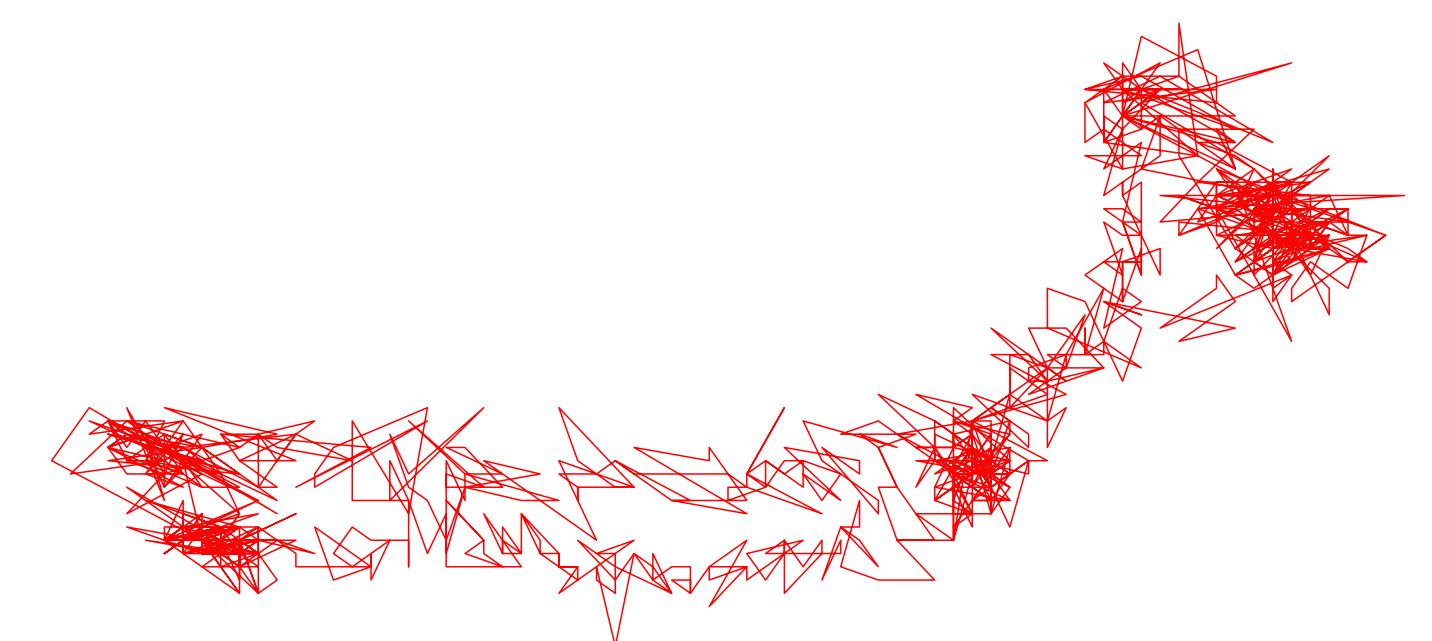
\includegraphics[width=30mm]{l0_particle_traj.png}}
\caption{Trajectory of data set 1 particle filter}
\end{figure} 

\begin{figure}[H]
\centerline{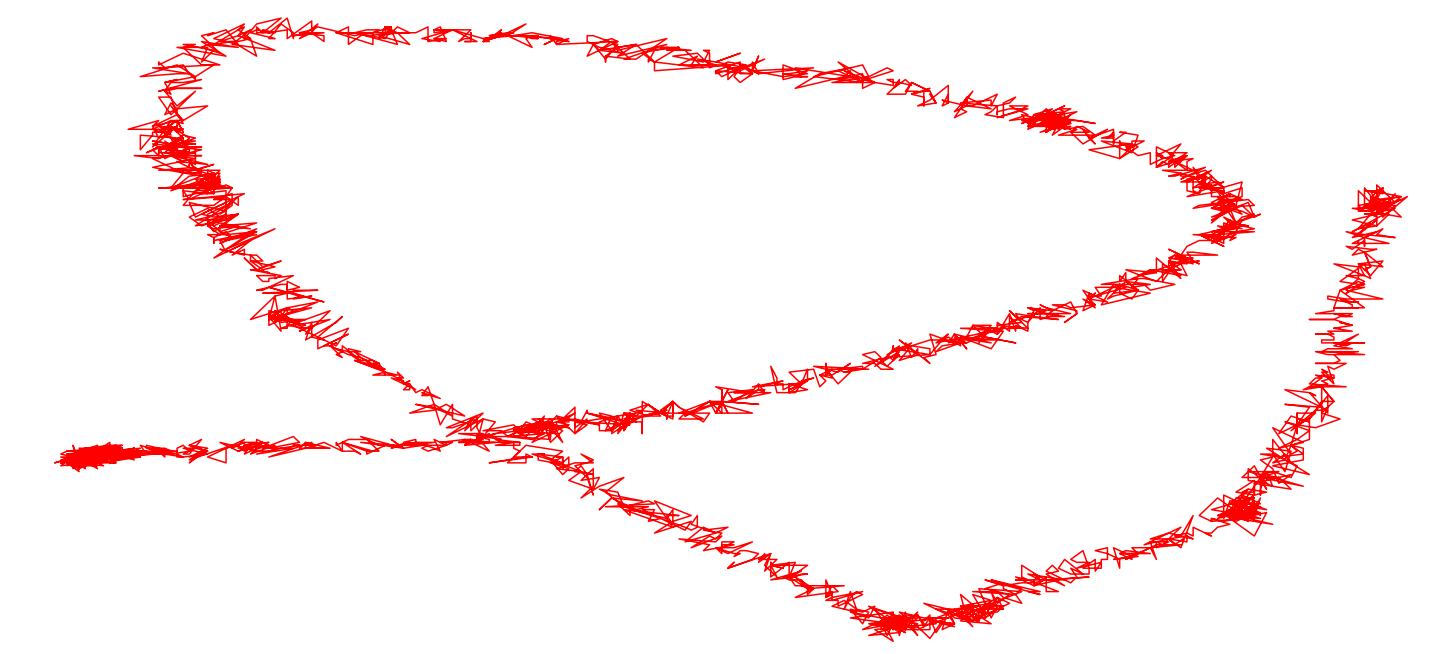
\includegraphics[width=30mm]{l1_particle_traj.png}}
\caption{Trajectory of data set 2 particle filter }
\end{figure}

\begin{figure}[H]
\centerline{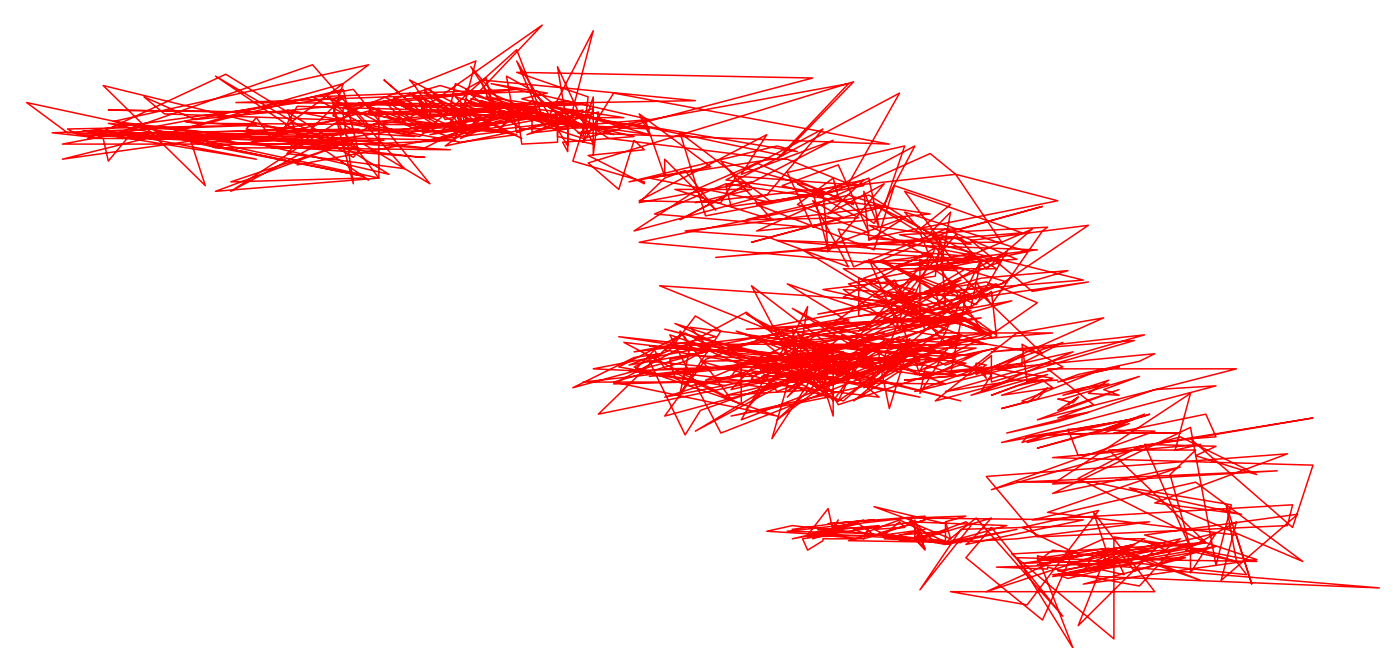
\includegraphics[width=30mm]{l2_particle_traj.png}}
\caption{Trajectory of data set 3 for particle filter}
\end{figure}

\begin{figure}[H]
\centerline{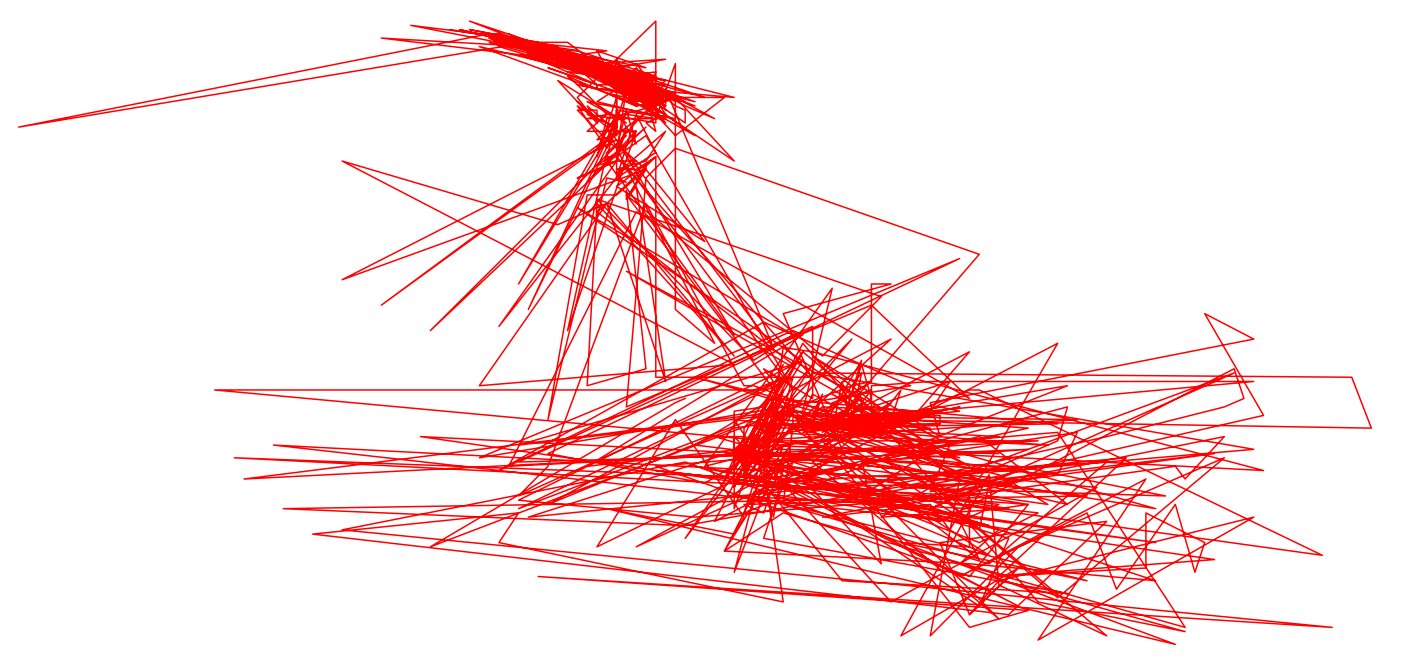
\includegraphics[width=30mm]{l3_particle_traj.png}}
\caption{Trajectory of data set 4 for particle filter}
\end{figure}

\begin{figure}[H]
\centerline{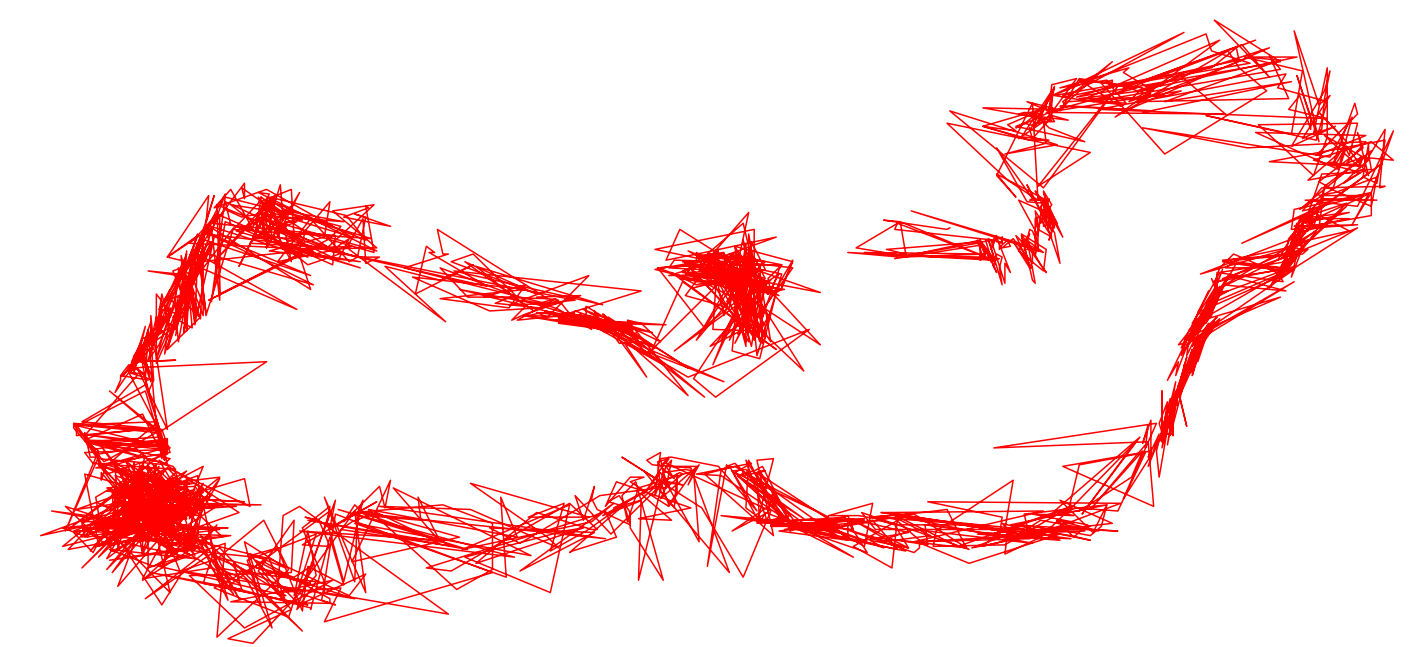
\includegraphics[width=30mm]{l4_particle_traj.png}}
\caption{Trajectory of data set 5 for particle filter}
\end{figure}



\begin{thebibliography}{00}
\bibitem{b1} https://natanaso.github.io/ece276a
\end{thebibliography}
\end{document}
